% !TeX root = ../../main.tex
\newpage
\section{Zbiory danych}

Do przeprowadzenia eksperymentów użyto dwóch zbiorów danych, w skład których wchodzą między innymi zdjęcia otrzymane od firmy ``BLUE''.
Jeden zbiór, zwany dalej zbiorem \textit{high} pochodzi z kamer ustawianych ponad kortem.
Drugi zbiór, zwany dalej zbiorem \textit{low}, pochodzi z kamer sytuowanych na podłodze, tuż przy liniach kortu.


\begin{figure}[!htb]
  \minipage{0.45\textwidth}
    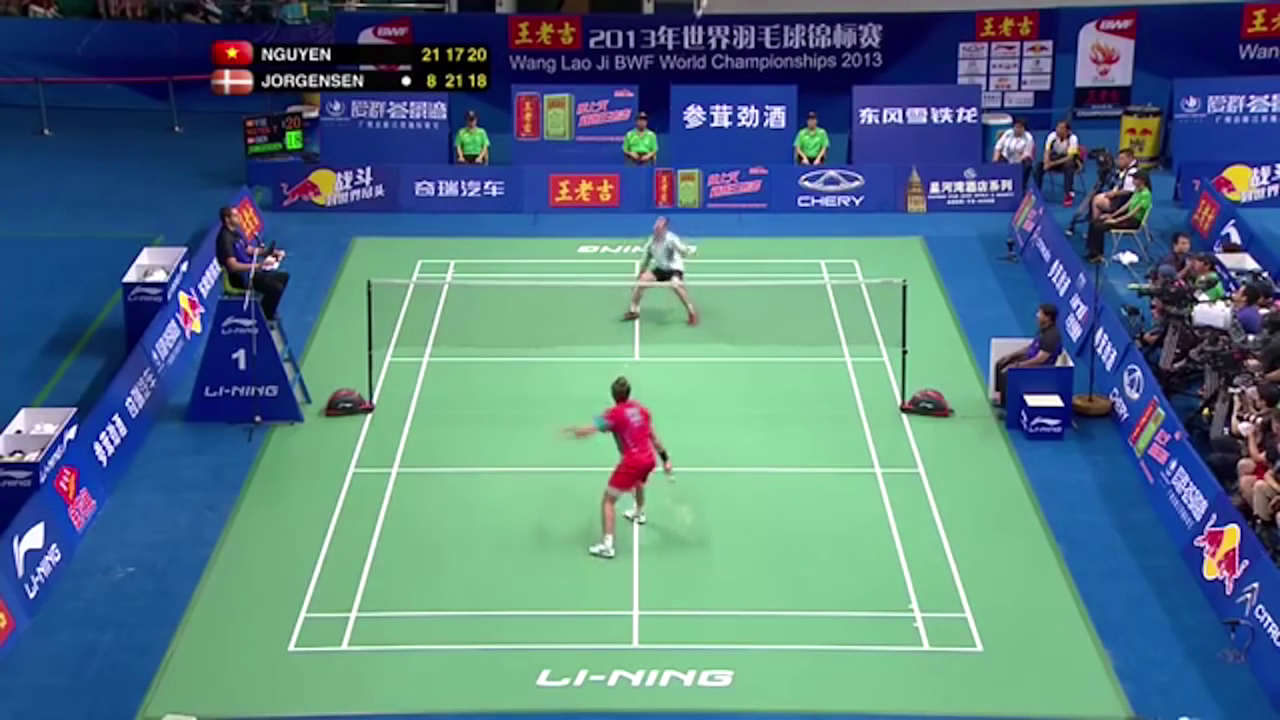
\includegraphics[width=\linewidth]{../../badminton/datasets/high/split/test_court2-00002.png}
    \caption{Przykładowy obraz ze zbioru danych \textit{high}}
  \endminipage\hfill
  \minipage{0.45\textwidth}
    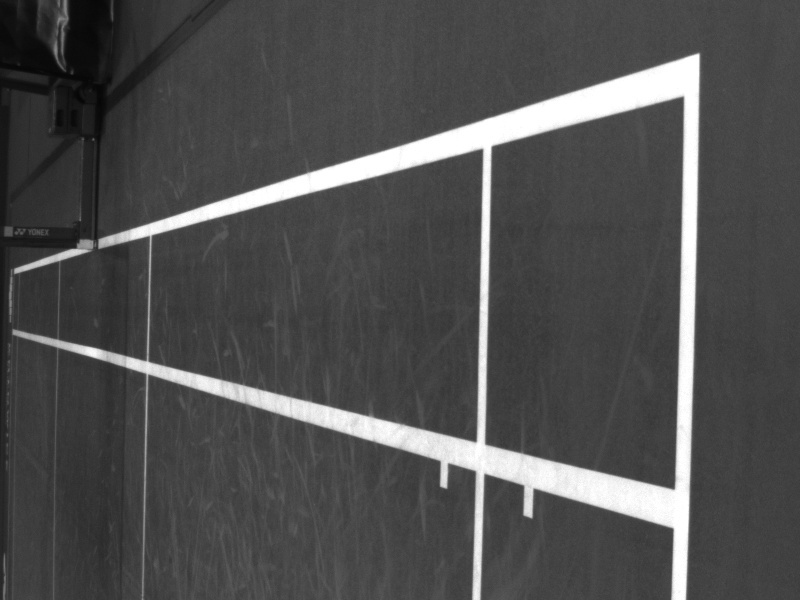
\includegraphics[width=\linewidth]{../../badminton/datasets/low/split/1564909032792410075.jpg}
    \caption{Przykładowy obraz ze zbioru danych \textit{low}}
  \endminipage\hfill
\end{figure}

Zbiór danych \textit{high} składa się z obrazów o różnych rozmiarach, i pochodzących z różnych źródeł.
Zbiór \textit{low} zawiera obrazy pozyskane wyłącznie od firmy ``BLUE'', o rozdzielczości 896x640 pikseli.
Zbiory podzielone są na podzbiory treningowe, walidacyjne oraz testowe w następujący sposób (wraz z porównaniem ze zbiorem COCO \cite{coco}):

\begin{table}[!h]
	\centering
	\caption{Liczba obrazów w podziale na poszczególne podzbiory}
	\vspace{6pt}
	{\footnotesize
		\begin{tabular}{|c|c|c|c|}
			\hline \textbackslash & Podzbiór treningowy & Podzbiór walidacyjny & Podzbiór testowy \\
      \hline Zbiór \textit{low} & 156 & 51 & 2 \\
      \hline Zbiór \textit{high} & 134 & 7 & 2 \\
      \hline Zbiór COCO & ok. 118000 & ok. 5000 & ok. 41000 \\
      \hline
		\end{tabular}
	}
	\vspace{0pt}
\end{table}

